\documentclass[11pt,letterpaper]{article}
\usepackage[margin=0.76in,headheight=15pt,headsep=14pt,footskip=28pt]{geometry}
\usepackage{newtxtext,newtxmath}
\usepackage{amsmath,enumitem,xcolor,tikz,fancyhdr}
\usepackage[colorlinks=true,urlcolor=blue!45!black,linkcolor=blue!45!black]{hyperref}
\usetikzlibrary{arrows.meta}
\definecolor{inkblue}{HTML}{24566D}
\setlength{\parindent}{0pt}
\setlength{\parskip}{7pt}
\setlength{\abovedisplayskip}{10pt}
\setlength{\belowdisplayskip}{10pt}
\setlist[enumerate]{leftmargin=1.6em,itemsep=6pt,topsep=4pt}
\pagestyle{fancy}
\fancyhf{}
\fancyhead[L]{Math 233H \quad Fall 2026}
\fancyhead[R]{Lecture 6: vector functions and motion}
\fancyfoot[C]{\thepage}
\renewcommand{\headrulewidth}{0.4pt}
\newcommand{\R}{\mathbf r}
\newcommand{\V}{\mathbf v}
\newcommand{\A}{\mathbf a}
\newcommand{\T}{\mathbf T}
\newcommand{\N}{\mathbf N}
\newcommand{\B}{\mathbf B}
\newcommand{\F}{\mathbf F}
\newcommand{\ii}{\mathbf i}
\newcommand{\jj}{\mathbf j}
\newcommand{\kk}{\mathbf k}
\newcommand{\norm}[1]{\left\lVert#1\right\rVert}
\newcommand{\heading}[1]{\vspace{5pt}{\large\bfseries #1}\par}
\newcommand{\subhead}[1]{\textbf{#1}\quad}
\hypersetup{pdftitle={Math 233H Lecture 6: vector functions and motion},pdfauthor={Jenia Tevelev},pdfsubject={Lecture 6: velocity, speed, arc length, integration, projectiles, acceleration, and the moving frame}}
\renewcommand*{\HyperDestNameFilter}[1]{lecture6-#1}
\begin{document}
\providecommand{\startpage}{1}
\setcounter{page}{\startpage}
{\LARGE\bfseries Lecture 6: vector functions and motion}\par
Jenia Tevelev \enspace$\cdot$\enspace Math 233H \enspace$\cdot$\enspace Fall 2026

Sections 13.3--13.4 connect the geometry of a curve with the motion of a particle. A vector function
\[
 \R(t)=\langle f(t),g(t),h(t)\rangle
       =f(t)\ii+g(t)\jj+h(t)\kk
\]
is the particle's position at time $t$; its image is the trajectory.

\heading{Velocity and speed}
The average velocity over a nonzero time increment $\Delta t$ is
\[
 \frac{\R(t+\Delta t)-\R(t)}{\Delta t}.
\]
Taking the limit as $\Delta t\to0$ gives the instantaneous velocity. Its magnitude is the speed:
\[
 \boxed{\V(t)=\R'(t),\qquad s(t)=\norm{\V(t)}.}
\]
Velocity is a vector; speed is a nonnegative scalar. A nonzero derivative also gives the direction of the tangent line to the trajectory.

\heading{Three examples}
\subhead{A line.} For
\[
 \R(t)=\langle1+t,1-2t,2+2t\rangle,
\]
we have $\V=\langle1,-2,2\rangle$ and $s=\sqrt{1+4+4}=3$. Both the velocity and the speed are constant.

\subhead{Circular motion.} Let $A>0$ be the radius and let $\omega$ be constant:
\[
 \R(t)=\langle A\cos(\omega t),A\sin(\omega t),0\rangle.
\]
Then
\[
 \V(t)=\langle-A\omega\sin(\omega t),A\omega\cos(\omega t),0\rangle,
 \qquad s=A|\omega|.
\]
For $\omega\ne0$, velocity changes direction even though speed is constant. The angular speed is $|\omega|$; when $\omega>0$, these quantities are $\omega$ and $A\omega$. The sign of $\omega$ determines the direction around the circle.

\subhead{The helix.} For
\[
 \R(t)=\langle\cos t,\sin t,t\rangle,
\]
the projection onto the $xy$-plane is a unit circle while the point rises along the $z$-axis. Here
\[
 \V(t)=\langle-\sin t,\cos t,1\rangle,
 \qquad s=\sqrt{\sin^2t+\cos^2t+1}=\sqrt2.
\]
The velocity changes direction, but the speed is constant.

\newpage
\heading{Arc length as accumulated distance}
The arc-length formula from the preceding lecture is
\[
 \boxed{L=\int_a^b\norm{\R'(t)}\,dt=\int_a^b s(t)\,dt.}
\]
The physical interpretation explains the formula: during a short time interval $\Delta t$, the particle travels approximately $s(t)\Delta t$. Add these short distances and refine the subdivision. The limiting sum is the integral of speed.

More explicitly, for a partition $a=t_0<t_1<\cdots<t_n=b$, the corresponding sum is
\[
 \sum_{j=1}^n s(\tau_j)(t_j-t_{j-1}),
 \qquad \tau_j\in[t_{j-1},t_j].
\]
For continuous speed these Riemann sums converge to $\int_a^b s(t)\,dt$ as the mesh tends to zero. This gives the distance traveled along the parametrized motion. Retracing part of the trajectory counts that distance again.

\subhead{Distance and displacement.} The small scalar $s(t)\Delta t$ approximates \emph{distance}, whereas the vector $\R'(t)\Delta t$ approximates \emph{displacement}. Thus
\[
 \int_a^b\norm{\R'(t)}\,dt\quad\hbox{is a scalar},
 \qquad
 \int_a^b\R'(t)\,dt=\R(b)-\R(a)\quad\hbox{is a vector}.
\]
Integrating a vector function component by component and computing arc length are different operations.

\heading{Separating speed from direction}
At a time when $\R'(t)\ne\mathbf0$, the \emph{unit tangent vector} is
\[
 \boxed{\T(t)=\frac{\R'(t)}{\norm{\R'(t)}}=\frac{\V(t)}{s(t)}.}
\]
It has length one and points in the direction of velocity. Consequently,
\[
 \boxed{\V(t)=s(t)\T(t).}
\]
The scalar $s$ records how fast the particle moves; $\T$ records its direction. This definition requires nonzero velocity: the zero vector has no direction, and division by its length would be division by zero.

\heading{Acceleration}
The rate of change of velocity is acceleration:
\[
 \boxed{\A(t)=\V'(t)=\R''(t).}
\]
Because velocity contains both speed and direction, acceleration can arise from a change in either one. This is why the circular and helical motions can have constant speed without constant velocity.

\newpage
\heading{Recovering position from acceleration}
Find the motion with
\[
 \A(t)=\cos t\,\ii+\sin t\,\jj+2t\,\kk,
 \qquad \V(0)=\jj,
 \qquad\R(0)=\langle1,0,2\rangle.
\]
Acceleration alone does not determine position: both the initial velocity and initial position are needed.

\subhead{Step 1: integrate to find velocity.} Integrate each component and include a constant \emph{vector} $\mathbf C$:
\[
 \V(t)=\sin t\,\ii-\cos t\,\jj+t^2\,\kk+\mathbf C.
\]
At $t=0$ this gives $\V(0)=-\jj+\mathbf C$. The initial condition $\V(0)=\jj$ therefore yields $\mathbf C=2\jj$, so
\[
 \boxed{\V(t)=\sin t\,\ii+(2-\cos t)\jj+t^2\kk.}
\]

\subhead{Step 2: integrate to find position.} Use a new constant vector $\mathbf D$:
\[
 \R(t)=-\cos t\,\ii+(2t-\sin t)\jj+\frac{t^3}{3}\kk+\mathbf D.
\]
At $t=0$ this is $-\ii+\mathbf D$. Thus
\[
 -\ii+\mathbf D=\langle1,0,2\rangle,
 \qquad \mathbf D=\langle2,0,2\rangle=2\ii+2\kk.
\]
The resulting position is
\[
 \boxed{\R(t)=(2-\cos t)\ii+(2t-\sin t)\jj+
             \left(2+\frac{t^3}{3}\right)\kk.}
\]
Differentiating twice recovers $\A$; substituting $t=0$ recovers both initial conditions.

\heading{Newton's second law}
For a particle of constant mass $m>0$, net force and acceleration satisfy
\[
 \boxed{\F=m\A.}
\]
If force is known as a function of time, division by $m$ gives acceleration. Two integrations, using initial velocity and position, reconstruct the motion:
\[
 \F(t)\ \longrightarrow\ \A(t)=\frac{\F(t)}m
 \ \longrightarrow\ \V(t)\ \longrightarrow\ \R(t).
\]
In the next example the gravitational acceleration is approximately constant. A force depending on the unknown position or velocity instead gives a differential equation; the two integrations need not then be independent antiderivatives of known time functions.

\newpage
\heading{Projectile motion under constant gravity}
Launch from the origin with initial speed $v_0>0$ at angle $0<\alpha<\pi/2$ above the horizontal. Assume constant downward gravity, no air resistance, and a landing surface at the launch height. Take $x$ horizontal and $y$ upward.
\[
 \A=\langle0,-g\rangle,\qquad
 \V(0)=\langle v_0\cos\alpha,v_0\sin\alpha\rangle,
 \qquad \R(0)=\langle0,0\rangle.
\]
Here $g>0$ is the magnitude of gravitational acceleration near Earth's surface, and $\F=\langle0,-mg\rangle$.

\begin{center}
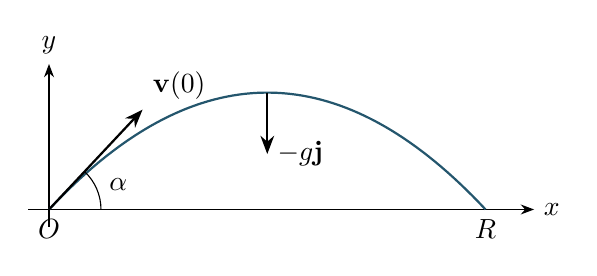
\begin{tikzpicture}[x=1.0cm,y=1.0cm,>=Stealth,scale=.88]
 \draw[->] (-.3,0)--(7.0,0) node[right] {$x$};
 \draw[->] (0,-.25)--(0,2.1) node[above] {$y$};
 \draw[inkblue,thick,domain=0:6.3,samples=70] plot (\x,{.17*\x*(6.3-\x)});
 \draw[->,thick] (0,0)--(1.35,1.44) node[above right] {$\V(0)$};
 \draw (.75,0) arc (0:46.85:.75);
 \node at (1.0,.36) {$\alpha$};
 \draw[->,thick] (3.15,1.687)--(3.15,.8) node[right] {$-g\jj$};
 \node[below] at (0,0) {$O$};
 \node[below] at (6.3,0) {$R$};
\end{tikzpicture}
\end{center}
\subhead{Velocity.} Integrating gives $\V(t)=\langle0,-gt\rangle+\mathbf C$. The initial condition fixes $\mathbf C=\V(0)$, hence
\[
 \V(t)=\langle v_0\cos\alpha,\ v_0\sin\alpha-gt\rangle.
\]
The horizontal velocity stays constant; the vertical velocity decreases.

\subhead{Position.} Integrating again and using $\R(0)=\mathbf0$ gives
\[
 \boxed{x(t)=v_0\cos\alpha\,t,\qquad
        y(t)=v_0\sin\alpha\,t-\frac12gt^2.}
\]
\subhead{Return to the ground.} Set $y(t)=0$:
\[
 t\left(v_0\sin\alpha-\frac12gt\right)=0.
\]
The solution $t=0$ is the launch time. The next contact with the ground occurs at
\[
 t_{\rm land}=\frac{2v_0\sin\alpha}{g}.
\]
\subhead{Horizontal range.} Substituting this time into $x(t)$ yields
\[
 \boxed{R=\frac{2v_0^2\sin\alpha\cos\alpha}{g}
           =\frac{v_0^2\sin(2\alpha)}g.}
\]
For fixed $v_0$, the range is greatest when $\sin(2\alpha)=1$, so $\alpha=\pi/4$. This conclusion uses the assumptions above, particularly equal launch and landing heights.

\newpage
\heading{Tangential and normal acceleration}
Return to $\V=s\T$ on an interval where the motion is twice continuously differentiable and $s>0$. The scalar--vector product rule gives
\[
 \A=\V'=s'\T+s\T'.
\]
The two terms are perpendicular. Indeed, $\T\cdot\T=1$, so
\[
 0=\frac{d}{dt}(\T\cdot\T)=2\T\cdot\T'.
\]
Thus $s'\T$ is the acceleration component along the tangent direction, while $s\T'$ is perpendicular to that direction.

\heading{The principal unit normal}
Where $\T'(t)\ne\mathbf0$, define
\[
 \boxed{\N(t)=\frac{\T'(t)}{\norm{\T'(t)}}.}
\]
Then $\N$ has length one and is perpendicular to $\T$. It records the direction in which the tangent turns. Replacing $\T'$ by $\norm{\T'}\N$ gives
\[
 \A=s'\T+s\norm{\T'}\N.
\]

\heading{Curvature}
The curvature is the rate at which the unit tangent changes per unit distance traveled:
\[
 \boxed{\kappa(t)=\frac{\norm{\T'(t)}}{\norm{\R'(t)}}
                         =\frac{\norm{\T'(t)}}{s(t)}.}
\]
Consequently, $\norm{\T'}=s\kappa$, and the acceleration decomposition becomes
\[
 \boxed{\A=s'\T+s^2\kappa\N.}
\]
Because $\T$ and $\N$ are perpendicular unit vectors, their coefficients give the tangential and normal scalar components:
\[
 \boxed{a_T=s',\qquad a_N=s^2\kappa.}
\]
The \emph{vector} components are $a_T\T$ and $a_N\N$. The tangential coefficient $a_T$ is signed: it is positive when speed increases and negative when speed decreases. The normal coefficient $a_N\ge0$ measures the acceleration that changes the direction of motion.

\subhead{Constant speed.} If speed is constant, $s'=0$, so the tangential component vanishes. Normal acceleration can still be nonzero.

\subhead{Domain of the definitions.} $\T$ requires $s>0$; $\N$ requires $\T'\ne\mathbf0$. At a regular point where $\T'=\mathbf0$, we still have $\kappa=0$ and $\A=s'\T$, but this definition does not supply a principal normal.

\newpage
\heading{Computing the curvature of the helix}
For the example used throughout the lecture,
\[
 \R(t)=\langle\cos t,\sin t,t\rangle,
 \qquad\R'(t)=\langle-\sin t,\cos t,1\rangle,
 \qquad s=\sqrt2.
\]
Normalize the velocity:
\[
 \T(t)=\frac1{\sqrt2}\langle-\sin t,\cos t,1\rangle.
\]
Differentiate the unit tangent, and then take its magnitude:
\[
 \T'(t)=\frac1{\sqrt2}\langle-\cos t,-\sin t,0\rangle,
 \qquad
 \norm{\T'(t)}=\frac1{\sqrt2}\sqrt{\cos^2t+\sin^2t}
              =\frac1{\sqrt2}.
\]
It follows that
\[
 \boxed{\kappa(t)=\frac{1/\sqrt2}{\sqrt2}=\frac12.}
\]
The curvature is the same everywhere along this helix. Its speed is also constant; these are different statements, concerning the motion and the bending of the trajectory, respectively.

\subhead{Normalization check.} The displayed $\T'$ and its length immediately give
\[
 \N(t)=\frac{\T'(t)}{\norm{\T'(t)}}=\langle-\cos t,-\sin t,0\rangle.
\]
This records the normalization needed to continue the frame calculation.

\heading{The binormal: introduced at the end of Lecture 6}
Where $\T$ and $\N$ are defined, their cross product is the \emph{binormal}:
\[
 \boxed{\B(t)=\T(t)\times\N(t).}
\]
It is perpendicular to both $\T$ and $\N$. Since those vectors are perpendicular and have length one, $\B$ also has length one. The order of the cross product fixes its orientation.

Acceleration is a linear combination of $\T$ and $\N$, so it belongs to the plane of directions they span. The binormal is perpendicular to that plane of directions.

The lecture began the helix calculation by setting up
\[
 \B(t)=\frac1{\sqrt2}\langle-\sin t,\cos t,1\rangle\times\N(t).
\]
\textbf{This calculation was not completed in Lecture 6.} Finishing the helix frame is part of the transition to the next lecture.

\heading{Where Lecture 7 begins}
We will return to the moving frame using Professor JT's rollercoaster demonstration and complete the geometric discussion, including the normal plane, osculating plane, and osculating circle. We will then begin the solar-system demonstration and Kepler's laws. These orbital laws were not started in Lecture 6.

\end{document}
